\documentclass{article}
\usepackage{graphicx}
\usepackage{titletoc}
\usepackage{titlesec}
\usepackage{geometry} 
\usepackage{fontspec, xunicode, xltxtra}
\usepackage{float}
\usepackage{cite}
\usepackage{amsmath}
\usepackage{listings}
\usepackage{titletoc}

\geometry{left=3cm,right=3cm,top=3cm,bottom=3cm}
\DeclareMathOperator*{\argmin}{argmin}
\DeclareMathOperator*{\argmax}{argmax}
\DeclareMathOperator*{\logit}{logit}
\DeclareMathOperator*{\var}{var}
\DeclareMathOperator*{\cov}{cov}
\DeclareMathOperator*{\expec}{E}
\DeclareMathOperator*{\deriv}{d}
\DeclareMathOperator*{\const}{constant}

\begin{document}
\title{\textsf{Homework 5 for Bayesian Data Analysis}}
\author{Fan JIN\quad (2015011506)}
\maketitle

\section*{Question 6.1a}
{
    Under the model assumption of identical effect for each group, we fix the hyperparameter $\tau=0$ in our normal hierarchical model. Plug it in and we obtain $\theta_j \sim N(7.7, 4.1^2)$. The posterior predictive distribution is simulated as follows: \\
    1) generate $\theta \sim N(7.7, 4.1^2)$, and \\
    2) generate $y_j^\mathrm{rep} \sim N(\theta, \sigma_j^2)$ for each $j$, followed by \\
    3) calculate the order stastistics out of $y_j^\mathrm{rep}$ for each $j$.

    The observed order statistics are approximately the order statistics calculated from the replicated simulations above. 
    \begin{figure}[H]
      \centering
      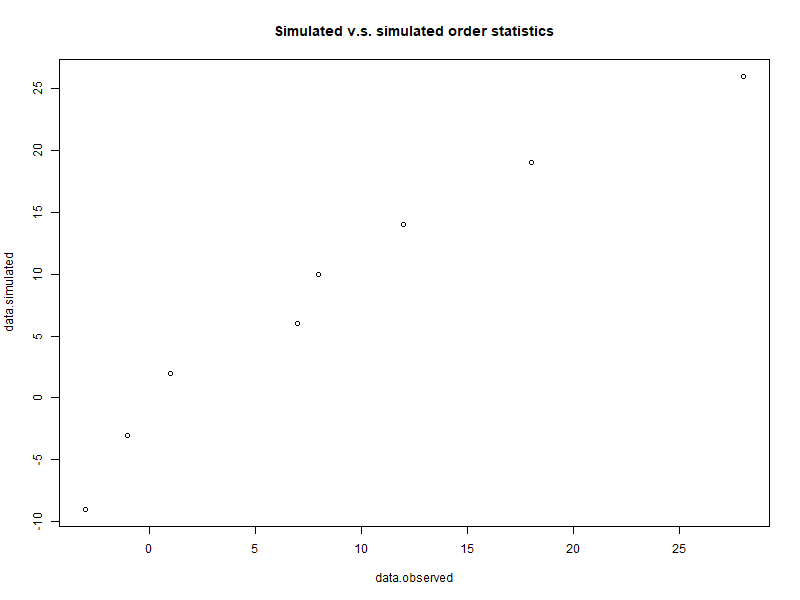
\includegraphics[width = 1.0\linewidth]{data.vs.png}
      \caption{Observed order statistics v.s. Simulations order statistics}
    \end{figure}
    \begin{lstlisting}
    > mod = lm((data.simulated - data.observed) ~ data.observed)
    > summary(mod)
    
    Call:
    lm(formula = (data.simulated - data.observed) ~ data.observed)
    
    Residuals:
        Min      1Q  Median      3Q     Max 
    -4.4555 -1.1794  0.3315  2.2663  2.6837 
    
    Coefficients:
                  Estimate Std. Error t value Pr(>|t|)
    (Intercept)   -1.30976    1.33122  -0.984    0.363
    data.observed  0.07826    0.10150   0.771    0.470
    
    Residual standard error: 2.805 on 6 degrees of freedom
    Multiple R-squared:  0.09014,	Adjusted R-squared:  -0.06151 
    F-statistic: 0.5944 on 1 and 6 DF,  p-value: 0.47
    \end{lstlisting}
    The p-value is 0.47, so the null hypothesis of unit slope cannot be rejected. We therefore conclude that the model fits the aspect of data here. 
}

\section*{Question 6.1b}
{
    The model of identical effect for each group assumes that $\theta_j = \theta$ for all $j$, and that school A has better effect than school C simply \emph{by chance}. But the model assumption can be skeptical given the observation, as we wonder whether there is other factors that cause school A to perform better than schoold C. In this case, the likelihood of the assumption of identical effects is far from being convincing, especially compared to the hierarchical models. 
}

\section*{Question 6.6a}
{
    We have 7 ones and 13 zeros out of the $n=20$ observations. 
    \begin{itemize}
        \item \textbf{Assume stops at 20th observation:}\quad The likelihood is proportional to $\theta^{7} (1-\theta)^{13}$, according to the binomial model with number of observations fixed to 20.
        \item \textbf{Assume stops at 13th zero:}\quad The likelihood is also proportional to $\theta^{7} (1-\theta)^{13}$, \emph{up to a different scale}, according to the negative binomial model with number of failures fixed to 13 with the last trial fixed to zero. 
    \end{itemize}
    There is no difference with the likelihood except for a constant factor. Therefore, the posterior distribution does not change, either.
}

\section*{Question 6.6b}
{
    Generate $\theta$ from $p(\theta) \sim \theta^{7} (1-\theta)^{13}$ for 10000 times, and generate $y^\mathrm{rep}$ under the new protocol (stops at the 13th zero) each time. 
    \begin{figure}[H]
        \centering
        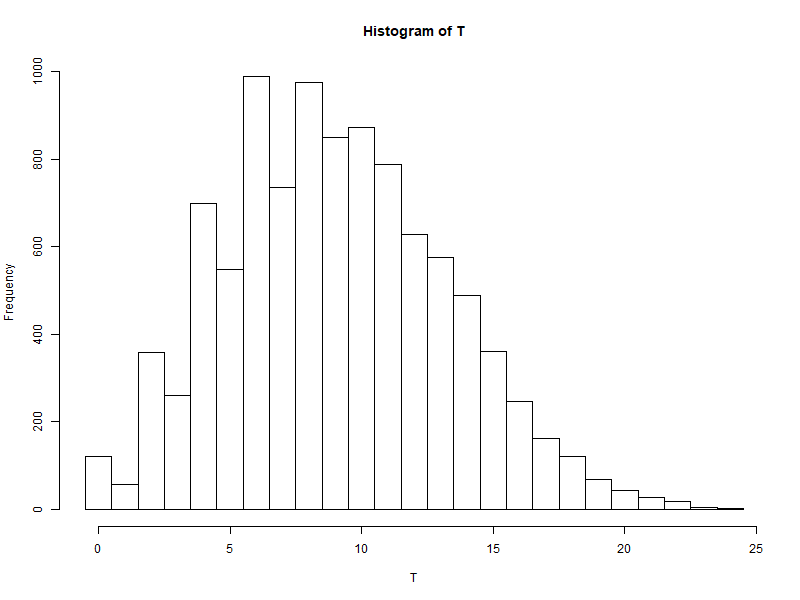
\includegraphics[width = 1.0\linewidth]{switches.histogram.png}
        \caption{Histogram of number of switches}
    \end{figure}

    First, the statistic T has a distribution with a heavier tail. This is because the number of observations can exceed the limit of $n=20$ under the new protocol. 

    Second, we find that T is more likely to be an even number than an odd number when $T < 10$. A possible explanation is: The last few observations must be zeros when $T$ is small, since the last one must be zero and there is few switches. Note that there must be $13$ zeros in total. Therefore, the distribution of $T$ is highly related to the specific value of $T$, i.e. $p(T=k)$ is more sensitive to $k$ when $k$ is relatively small. 
}

\section*{Source Code in R}
{
    \begin{lstlisting}[language=R]
    # Question 6.1
    data.observed = c(28, 18, 12, 8, 7, 1, -1, -3)
    data.simulated = c(26, 19, 14, 10, 6, 2, -3, -9)
    
    png("data.vs.png", width=800, height=600)
    plot(data.observed, data.simulated, main="Simulated v.s. simulated order statistics")
    dev.off()
    
    mod = lm((data.simulated - data.observed) ~ data.observed)
    summary(mod)
    
    
    # Question 6.6
    T0 = 3 # number of switches
    N = 10000
    T = 1:N
    theta = rbeta(N, shape1=7+1, shape2=13+1)
    for (j in 1:N) {
        count.switches = 0
        y.last = rbinom(1, size=1, prob=theta[j])
        count.zeros = 1 - y.last
        while (1) {
        y = rbinom(1, size=1, prob=theta[j])
        if (y != y.last) {
            count.switches = count.switches + 1
        }
        count.zeros = count.zeros + 1 - y.last
        if (count.zeros > 12.5) {
            break;
        }
        y.last = y
        }
        T[j] = count.switches
    }
    png("switches.histogram.png", width=800, height=600)
    hist(T, breaks=seq(-0.5, max(T)+0.5))
    dev.off()
    \end{lstlisting}
}

\clearpage
\end{document}
